\section{Πλήρης Κάλυψη Χάρτη}
\label{sec:experiments_coverage}

Το τρίτο και μεγαλύτερο μέρος των πειραμάτων περιέχει την πλήρη κάλυψη ενός χώρου. Στα πλαίσια της μελέτης αυτής χρησιμοποιήθηκαν τρεις διαφορετικοί χάρτες με διαφορετικό επίπεδο πολυπλοκότητας περιβάλλοντος, όπως φαίνεται στα αντίστοιχα OGM \ref{fig:experiments_maps}. Ο πρώτος χάρτης αποτελεί ένα πολύ απλό περιβάλλον δύο μικρών δωματίων, ο δεύτερος ένα άδειο περιβάλλον με 5 δωμάτια και ο τρίτος ένα πολύπλοκο περιβάλλον με 6 δωμάτια και πολλά εμπόδια.


\begin{figure}
     \centering
     \begin{subfigure}[b]{\textwidth}
         \centering
         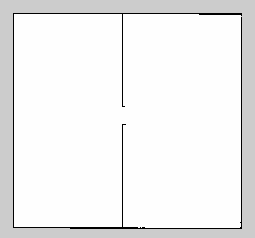
\includegraphics[width=0.4\textwidth]{./images/chapter6/map_a_ogm.png}
         \label{fig:map_a_ogm}
         \caption{Χάρτης map\_a}
     \end{subfigure}
     \hfill
     \begin{subfigure}[b]{\textwidth}
         \centering
         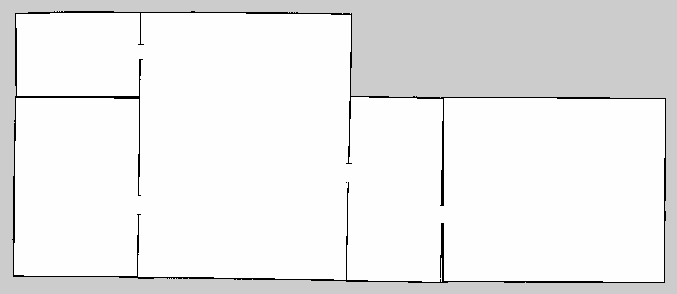
\includegraphics[width=0.6\textwidth]{./images/chapter6/rooms_3_ogm.png}
         \label{fig:rooms_3_ogm}
         \caption{Χάρτης rooms\_3}
     \end{subfigure}
     \hfill
     \begin{subfigure}[b]{\textwidth}
         \centering
         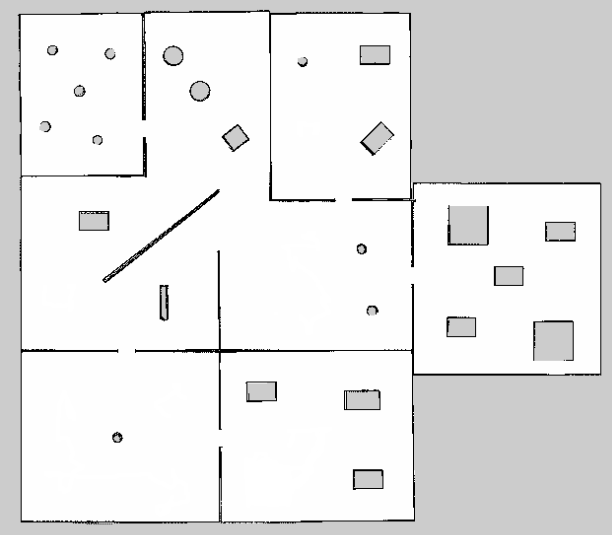
\includegraphics[width=0.6\textwidth]{./images/chapter6/indoors_with_features_ogm.png}
         \label{fig:indoors_with_features_ogm}
         \caption{Χάρτης indoors\_with\_features}
     \end{subfigure}
    \caption{Περιβάλλοντα που χρησιμοποιήθηκαν στα πειράματα κάλυψης χώρου}
    \label{fig:experiments_maps}
\end{figure}

Στην μελέτη χρησιμοποιήθηκαν 4 διαφορετικά σετ αισθητήρων για την πλήρη προσομοίωση όλων των πιθανών περιπτώσεων. Σε όλες τις περιπτώσεις τοποθετήθηκαν δύο κεραίες στα πλάγια μέρη του οχήματος. Αυτά είναι:

\begin{table}[H]
    \begin{center}
        \caption{Παράμετροι αισθητήρων RFID}
        \label{tab:rfid_configs}
        \begin{tabular}{ | c | c | c | c |}
        \hline
        \rowcolor{Gray}
        Τύπος & FOV & Εύρος\\
        Ευρύ FOV - Μικρή Ακτίνα & \ang{70} &  1 \si{m} \\ 
        Ευρύ FOV - Μεγάλη Ακτίνα & \ang{70} &  3 \si{m} \\
        Στενό FOV - Μικρή Ακτίνα & \ang{35} &  1 \si{m} \\
        Στενό FOV - Μεγάλη Ακτίνα & \ang{35} &  3 \si{m} \\
        
        \hline
        \end{tabular}
    \end{center}
\end{table}

Τέλος, χρησιμοποιήθηκαν 4 διαφορετικές στρατηγικές δημιουργίας των αντίστοιχων μονοπατιών κάλυψης του κάθε χώρου, οι οποίες είναι:
\begin{itemize}
    \setlength\itemsep{-0.2em}
    \item Στρατηγική Ακολουθίας Τοίχων (Wall Follow)
    \item Στρατηγική Ζιγκ Ζαγκ
    \item Απλή Στρατηγική με Δειγματοληψία μικρού σταθερού βήματος
    \item Απλή Στρατηγική με Δειγματοληψία μεγάλου σταθερού βήματος
\end{itemize}
Οι δύο πρώτες αποτελούν τις δύο στρατηγικές που υλοποιήθηκαν στον κορμό της παρούσας διπλωματικής εργασία. Οι δύο τελευταίες αποτελούν μια απλοποιημένη εκδοχή των προηγούμενων μεθόδων, ώστε να μελετηθεί εαν η πολυπλοκότητα των υπολογισμών πράγματι βοηθάει στο αποτέλεσμα.

Οι απλές στρατηγικές αποτελούνται από μια ομοιόμορφη δειγματοληψία σημείων σταθερού βήματος, RRHC στην αλληλουχία κάθε δωματίου με σταθερά άκρα, τις πόρτες εισόδου και εξόδου του δωματίου και, τέλος, επιλογή του καλύτερου προσανατολισμού σε κάθε σημείο με τη χρήση του motor schema που υλοποιήθηκε με ίσα βάρη. Το μικρό βήμα δειγματοληψίας τέθηκε ίσο με 0.5 μέτρα και το μεγάλο με 2 μέτρα.

Σε κάθε κάλυψη συλλέγονται οι παρακάτω μετρήσεις:
\begin{itemize}
    \setlength\itemsep{-0.2em}
    \item Πλήθος poses διαδρομής
    \item Μήκος συνολικής διαδρομής
    \item Χρόνος πλήρους κάλυψης
    \item Ποσοστό συνολικής κάλυψης των εμποδίων του χώρου
    \item Μέση τιμή πλήθους σαρώσεων κάθε σημείου (mean of scans)
    \item Διακύμανση πλήθους σαρώσεων κάθε σημείου (std of scans)
    \item Μέση τιμή μετρικής γωνίας σάρωσης κάθε σημείου που έχει σαρωθεί (mean of scans' angles)
    \item Διακύμανση μετρικής γωνίας σάρωσης κάθε σημείου που έχει σαρωθεί (std of scans' angles)
\end{itemize}

Οι επόμενοι πίνακες παρουσιάζουν τα αποτελέσματα από το σύνολο των πειραμάτων χωρισμένα ανά χάρτη και για όλα τα σετ αισθητήρων.


\begin{table}[H]
  \begin{center}
    \caption{Αποτελέσματα στον map\_a με Ευρύ FOV - Μικρή Ακτίνα}
    \label{tab:map_a_i_results}
    \begin{tabular}{ |>{\columncolor[gray]{0.8}}  c | c | c | c | c |}
      \hline
      \rowcolor{gray}
      Στρατηγική & Wall Follow & Zig Zag & Simple small & Simple Large \\
      Number of Poses & $150$ & $233$ & $126$ & $10$ \\ \hline
      Total path length & $1287.97$ & $1576.87$ & $1169.17$ & $452.03$ \\ \hline
      Total time (secs) & $1335$ & $1910$ & $773$ & $97$ \\ \hline
      Coverage percentage & $100$\% & $99.84$\% & $99.29$\% & $6.07$\% \\ \hline
      Mean of scans & $17.7743$ & $30.6754$ & $10.5984$ & $0.5719$ \\ \hline
      Std of scans & $11.5988$ & $17.6976$ & $6.5329$ & $2.605$ \\ \hline
      Mean of scans' angles & $0.43401$ & $0.35269$ & $0.2936$ & $0.1451$ \\ \hline
      Std of scans' angles  & $0.49562$ & $0.4778$ & $0.4554$ & $0.3522$ \\ 
      \hline
    \end{tabular}
  \end{center}
\end{table}

\begin{table}[H]
  \begin{center}
    \caption{Αποτελέσματα στον map\_a με Ευρύ FOV - Μεγάλη Ακτίνα}
    \label{tab:map_a_ii_results}
    \begin{tabular}{ |>{\columncolor[gray]{0.8}}  c | c | c | c | c |}
      \hline
      \rowcolor{gray}
      Στρατηγική & Wall Follow & Zig Zag & Simple small & Simple Large \\
      Number of Poses & $20$ & $43$ & $126$ & $10$ \\ \hline
      Total path length & $809.612$ & $971.98$ & $1169.17$ & $452.03$ \\ \hline
      Total time (secs) & $310$ & $501$ & $855$ & $101$ \\ \hline
      Coverage percentage & $99.7$\% & $99.688$\% & $100$\% & $37.74$\% \\ \hline
      Mean of scans & $19.7494$ & $30.0677$ & $29.21167$ & $4.9159$ \\ \hline
      Std of scans & $9.8338$ & $15.84533$ & $20.5956$ & $7.8433$ \\ \hline
      Mean of scans' angles & $0.376$ & $0.35031$ & $0.2711$ & $0.2284$ \\ \hline
      Std of scans' angles  & $0.4843$ & $0.47706$ & $0.4453$ & $0.4198$ \\ 
      \hline
    \end{tabular}
  \end{center}
\end{table}


\begin{table}[H]
  \begin{center}
    \caption{Αποτελέσματα στον map\_a με Στενό FOV - Μικρή Ακτίνα}
    \label{tab:map_a_iii_results}
    \begin{tabular}{ |>{\columncolor[gray]{0.8}}  c | c | c | c | c |}
      \hline
      \rowcolor{gray}
      Στρατηγική & Wall Follow & Zig Zag & Simple small & Simple Large \\
      Number of Poses & $215$ & $297$ & $126$ & $10 $\\ \hline
      Total path length & $1268.06$ & $1557.15$ & $1169.17$ & $452.03$ \\ \hline
      Total time (secs) & $1620$ & $2898$ & $789$ & $106$ \\ \hline
      Coverage percentage & $100$\% & $99.53$\% & $99.221$\% & $5.83$\% \\ \hline
      Mean of scans & $14.5$ & $21.17665$ & $6.01634$ & $0.298$ \\ \hline
      Std of scans & $9.4428$ & $11.9857$ & $4.5871$ & $1.393$ \\ \hline
      Mean of scans' angles & $0.69623$ & $0.59139$ & $0.62365$ & $0.5636$ \\ \hline
      Std of scans' angles  & $0.45988$ & $0.49157$ & $0.48446$ & $0.4959$ \\ 
      \hline
    \end{tabular}
  \end{center}
\end{table}

\begin{table}[H]
  \begin{center}
    \caption{Αποτελέσματα στον map\_a με Στενό FOV - Μεγάλη Ακτίνα}
    \label{tab:map_a_iiv_results}
    \begin{tabular}{ |>{\columncolor[gray]{0.8}}  c | c | c | c | c |}
      \hline
      \rowcolor{gray}
      Στρατηγική & Wall Follow & Zig Zag & Simple small & Simple Large \\
      Number of Poses & $46$ & $60$ & $126$ & $10$ \\ \hline
      Total path length & $809.612$ & $971.98$ & $1169.17$ & $452.03$ \\ \hline
      Total time (secs) & $517$ & $618$ & $833$ & $96$ \\ \hline
      Coverage percentage & $99.92$\% & $99.61$\% & $100$\% & $37.66$\% \\ \hline
      Mean of scans & $15.3517$ & $19.4023$ & $15.5097$ & $2.785$ \\ \hline
      Std of scans & $6.5877$ & $9.2672$ & $12.0028$ & $4.744$ \\ \hline
      Mean of scans' angles & $0.5591$ & $0.3301$ & $0.53505$ & $0.3198$ \\ \hline
      Std of scans' angles  & $0.4964$ & $0.47025$ & $0.49876$ & $0.4664$ \\ 
      \hline
    \end{tabular}
  \end{center}
\end{table}

% -------------------------------------------------------------------


\begin{table}[H]
  \begin{center}
    \caption{Αποτελέσματα στον rooms\_3 με Ευρύ FOV - Μικρή Ακτίνα}
    \label{tab:rooms_3_i_results}
    \begin{tabular}{ |>{\columncolor[gray]{0.8}}  c | c | c | c | c |}
      \hline
      \rowcolor{gray}
      Στρατηγική & Wall Follow & Zig Zag & Simple small & Simple Large \\
      Number of Poses & $370$ & $572$ & $286$ & $30$ \\ \hline
      Total path length & $3875.882$ & $4537.929$ & $3490.03$ & $1627.56$ \\ \hline
      Total time (secs) & $3580$ & $5524$ & $2808$ & $408$ \\ \hline
      Coverage percentage & $98.91$\% & $98.396$\% & $97.881$\% & $12.25$\% \\ \hline
      Mean of scans & $14.38819$ & $19.8414$ & $10.6211$ & $0.8323$ \\ \hline
      Std of scans & $10.0359$ & $14.5949$ & $6.6085$ & $2.7883$ \\ \hline
      Mean of scans' angles & $0.43892$ & $0.42213$ & $0.44157$ & $0.47$ \\ \hline
      Std of scans' angles  & $0.49599$ & $0.4939$ & $0.49657$ & $0.4991$ \\ 
      \hline
    \end{tabular}
  \end{center}
\end{table}

\begin{table}[H]
  \begin{center}
    \caption{Αποτελέσματα στον rooms\_3 με Ευρύ FOV - Μεγάλη Ακτίνα}
    \label{tab:rooms_3_ii_results}
    \begin{tabular}{ |>{\columncolor[gray]{0.8}}  c | c | c | c | c |}
      \hline
      \rowcolor{gray}
      Στρατηγική & Wall Follow & Zig Zag & Simple small & Simple Large \\
      Number of Poses & $81$ & $114$ & $286$ & $30$ \\ \hline
      Total path length & $2562.367$ & $2968.296$ & $3490.03$ & $1627.56$ \\ \hline
      Total time (secs) & $1095$ & $1350$ & $2550$ & $405$ \\ \hline
      Coverage percentage & $98.577$\% & $98.638$\% & $99$\% & $59.45$\% \\ \hline
      Mean of scans & $21.6901$ & $28.3939$ & $31.47261$ & $6.146$ \\ \hline
      Std of scans & $13.7954$ & $16.8131$ & $13.2472$ & $7.338$ \\ \hline
      Mean of scans' angles & $0.35177$ & $0.304012$ & $0.29845$ & $0.4266$ \\ \hline
      Std of scans' angles  & $0.47752$ & $0.45998$ & $0.457581$ & $0.4945$ \\ 
      \hline
    \end{tabular}
  \end{center}
\end{table}


\begin{table}[H]
  \begin{center}
    \caption{Αποτελέσματα στον rooms\_3 με Στενό FOV - Μικρή Ακτίνα}
    \label{tab:rooms_3_iii_results}
    \begin{tabular}{ |>{\columncolor[gray]{0.8}}  c | c | c | c | c |}
      \hline
      \rowcolor{gray}
      Στρατηγική & Wall Follow & Zig Zag & Simple small & Simple Large \\
      Number of Poses & $473$ & $692$ & $286$ & $30$ \\ \hline
      Total path length & $3972.408$ & $4687.32$ & $3490.03$ & $1627.56$ \\ \hline
      Total time (secs) & $4125$ & $8682$ & $3157$ & $352$ \\ \hline
      Coverage percentage & $98.15$\% & $95.34$\% & $95.521$\% & $11.49$\% \\ \hline
      Mean of scans & $9.729$ & $10.0599$ & $5.43721$ & $0.4127$ \\ \hline
      Std of scans & $7.051$ & $9.1189$ & $3.96784$ & $1.458$ \\ \hline
      Mean of scans' angles & $0.7326$ & $0.63012$ & $0.72391$ & $0.796$ \\ \hline
      Std of scans' angles  & $0.4425$ & $0.48277$ & $0.44705$ & $0.4029$ \\ 
      \hline
    \end{tabular}
  \end{center}
\end{table}

\begin{table}[H]
  \begin{center}
    \caption{Αποτελέσματα στον rooms\_3 με Στενό FOV - Μεγάλη Ακτίνα}
    \label{tab:rooms_3_iiv_results}
    \begin{tabular}{ |>{\columncolor[gray]{0.8}}  c | c | c | c | c |}
      \hline
      \rowcolor{gray}
      Στρατηγική & Wall Follow & Zig Zag & Simple small & Simple Large \\
      Number of Poses & $126$ & $160$ & $286$ & $30$ \\ \hline
      Total path length & $2560.6$ & $3024.52$ & $3490.06$ & $1627.56$ \\ \hline
      Total time (secs) & $1301$ & $1978$ & $3133$ & $411$ \\ \hline
      Coverage percentage & $98.033$\% & $97.881$\% & $99.031$\% & $55.91$\% \\ \hline
      Mean of scans & $14.2375$ & $14.8172$ & $15.4$ & $3.138$ \\ \hline
      Std of scans & $8.5554$ & $8.9399$ & $7.8128$ & $4.059$ \\ \hline
      Mean of scans' angles & $0.43052$ & $0.43306$ & $0.61159$ & $0.4821$ \\ \hline
      Std of scans' angles  & $0.49514$ & $0.4954$ & $0.4873$ & $0.4996$ \\ 
      \hline
    \end{tabular}
  \end{center}
\end{table}


% -------------------------------------------------------------------




\begin{table}[H]
  \begin{center}
    \captionsetup{justification=centering}
    \caption{Αποτελέσματα στον indoors\_with\_features με Ευρύ FOV - Μικρή Ακτίνα}
    \label{tab:indoors_with_features_i_results}
    \begin{tabular}{ |>{\columncolor[gray]{0.8}}  c | c | c | c | c |}
      \hline
      \rowcolor{gray}
      Στρατηγική & Wall Follow & Zig Zag & Simple small & Simple Large \\
      Number of Poses & $608$ & $944$ & $743$ & $46$ \\ \hline
      Total path length & $8393.4909$$ & $9919.85$ & $10007.63$ & $2883.37$ \\ \hline
      Total time (secs) & $9047$ & $10715$ & $7808$ & $998$ \\ \hline
      Coverage percentage & $92.74$\% & $94.628$\% & $91.9$\% & $14.31$\% \\ \hline
      Mean of scans & $8.2309$ & $10.917$ & $8.94$ & $0.827$ \\ \hline
      Std of scans & $8.9038$ & $10.3473$ & $7.569$ & $2.55$ \\ \hline
      Mean of scans' angles & $0.487172$ & $0.42139$ & $0.3862$ & $0.5881$ \\ \hline
      Std of scans' angles  & $0.49983$ & $0.49377$ & $0.4868$ & $0.4921$ \\ 
      \hline
    \end{tabular}
  \end{center}
\end{table}

\begin{table}[H]
  \begin{center}
    \captionsetup{justification=centering}
    \caption{Αποτελέσματα στον indoors\_with\_features με Ευρύ FOV - Μεγάλη Ακτίνα}
    \label{tab:indoors_with_features_ii_results}
    \begin{tabular}{ |>{\columncolor[gray]{0.8}}  c | c | c | c | c |}
      \hline
      \rowcolor{gray}
      Στρατηγική & Wall Follow & Zig Zag & Simple small & Simple Large \\
      Number of Poses & $245$ & $316$ & $743$ & $46$ \\ \hline
      Total path length & $5241.9$ & $5972.02$ & $10007.63$ & $2883.37$ \\ \hline
      Total time (secs) & $3390$ & $4619$ & $7939$ & $972$ \\ \hline
      Coverage percentage & $96.901$\% & $96.801$\% & $96.49$\% & $60.21$\% \\ \hline
      Mean of scans & $27.6053$ & $32.8307$ & $41.6034$ & $7.385$ \\ \hline
      Std of scans & $10.4321$ & $21.0289$ & $28.9465$ & $8.907$ \\ \hline
      Mean of scans' angles & $0.283$ & $0.3033$ & $0.2055$ & $0.5$ \\ \hline
      Std of scans' angles  & $0.45048$ & $0.4597$ & $0.4041$ & $0.49$ \\ 
      \hline
    \end{tabular}
  \end{center}
\end{table}


\begin{table}[H]
  \begin{center}
    \captionsetup{justification=centering}
    \caption{Αποτελέσματα στον indoors\_with\_features με Στενό FOV - Μικρή Ακτίνα}
    \label{tab:indoors_with_features_iii_results}
    \begin{tabular}{ |>{\columncolor[gray]{0.8}}  c | c | c | c | c |}
      \hline
      \rowcolor{gray}
      Στρατηγική & Wall Follow & Zig Zag & Simple small & Simple Large \\
      Number of Poses & $820$ & $1179$ & $743$ & $46$ \\ \hline
      Total path length & $8479.88$ & $10105.16$ & $10007.63$ & $2883.37$ \\ \hline
      Total time (secs) & $10651$ & $15268$ & $7898$ & $977$ \\ \hline
      Coverage percentage & $92.916$\% & $91.267$\% & $96.72$\% & $56.35$\% \\ \hline
      Mean of scans & $6.42698$ & $6.25858$ & $21.4439$ & $3.823$ \\ \hline
      Std of scans & $5.8097$ & $6.14225$ & $16.4325$ & $5.1012$ \\ \hline
      Mean of scans' angles & $0.64802$ & $0.6669$ & $0.4615$ & $0.607$ \\ \hline
      Std of scans' angles  & $0.47758$ & $0.47131$ & $0.4985$ & $0.4484$ \\ 
      \hline
    \end{tabular}
  \end{center}
\end{table}

\begin{table}[H]
  \begin{center}
    \captionsetup{justification=centering}
    \caption{Αποτελέσματα στον indoors\_with\_features με Στενό FOV - Μεγάλη Ακτίνα}
    \label{tab:indoors_with_features_iv_results}
    \begin{tabular}{ |>{\columncolor[gray]{0.8}}  c | c | c | c | c |}
      \hline
      \rowcolor{gray}
      Στρατηγική & Wall Follow & Zig Zag & Simple small & Simple Large \\
      Number of Poses & $344$ & $419$ & $743$ & $46$ \\ \hline
      Total path length & $5097.26$ & $5841.74$ & $10007.63$ & $2883.37$ \\ \hline
      Total time (secs) & $4172$ & $5720$ & $7751$ & $942$ \\ \hline
      Coverage percentage & $96.327$\% & $96.664$\% & $86.95$\% & $13.7$\% \\ \hline
      Mean of scans & $16.4983$ & $18.7782$ & $4.6193$ & $0.4473$ \\ \hline
      Std of scans & $10.6672$ & $12.91$ & $4.21$ & $1.447$ \\ \hline
      Mean of scans' angles & $0.45$ & $0.5121$ & $0.6484$ & $0.7263$ \\ \hline
      Std of scans' angles  & $0.49749$ & $0.4998$ & $0.4774$ & $0.4458$ \\ 
      \hline
    \end{tabular}
  \end{center}
\end{table}


Αρχικά, παρατηρείται ότι η χρήση κεραιών RFID με μεγάλη ακτίνα και ευρύ πεδίο όρασης είναι η καλύτερη δυνατή, διότι οδηγεί σε πιο ικανοποιητικά αποτελέσματα. Πρώτον, μειώνει σημαντικά το χρόνο της συνολική κάλυψης του χώρου, καθώς απαιτούνται πολύ λιγότεροι στόχοι. Δεύτερον αυξάνει το μέσο όρο σαρώσεων ανά σημείο συγκριτικά με τις υπολοίπες κεραίες, διότι σαρώνονται συνεχώς περισσότερα τμήματα του χώρου. Τρίτον, στις δύο πρώτες στρατηγικές μειώνει τη μετρική γωνίας σάρωσης κάθε σημείου, δηλαδή η κάλυψη των εμποδίων γίνεται πιο ομοιόμορφα από τα δύο εύρη γωνιών. Όλες οι συγκρίσεις παρουσιάζονται και στα επόμενα γραφήματα \ref{fig:sensors_compare}. Με μπλε είναι η σύγκριση του αριθμού των στόχων, με κόκκινο του χρόνου πλοήγησης σε κάθε χάρτη, με πορτοκαλί της μέσης τιμής του αριθμού σαρώσεων των σημείων και με πράσινο της μέσης τιμής της μετρικής της γωνίας σάρωσης. Η σύγκριση γίνεται μεταξύ των τεσσάρων σετ αισθητήρων σε κάθε χάρτη και σε όλες τις περιπτώσεις παρατηρείται μικρότερος αριθμός στόχων, χρόνου και μετρικής γωνίας και μεγαλύτερη μέση τιμή σαρώσεων όταν χρησιμοποιούνται κεραίες με ευρύ FOV και μεγάλη ακτίνα. Σημειώνεται ότι τα αποτελέσματα αυτά αφορούν τη στρατηγική ακολουθίας τοίχων, η οποία είναι και η βασική στρατηγική της μελέτης αυτής. 

Επιπλέον, στο \autoref{fig:indoors_with_features_wall_follow_sensors_coverage_complare} παρουσιάζεται η τελική πλήρης κάλυψη του χάρτη από τα δύο διαφορετικά σετ αισθητήρων χρησιμοποιώντας τη στρατηγική ακολουθίας τοίχων.


\begin{figure}[H]
     \centering
     \captionsetup{justification=centering}
     \begin{subfigure}[b]{0.5\textwidth}
         \centering
         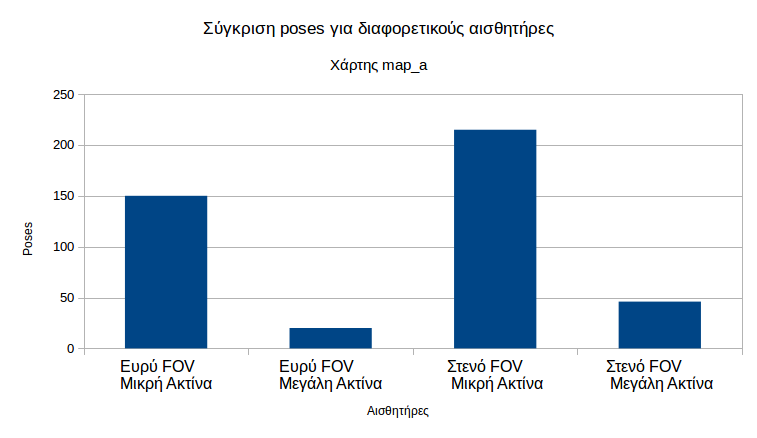
\includegraphics[width=\textwidth]{./images/chapter6/map_a_poses_compare.png}
         \label{fig:map_a_poses_compare}
         \caption{Σύγκριση αριθμών poses στον map\_a}
     \end{subfigure}%
     \begin{subfigure}[b]{0.5\textwidth}
         \centering
         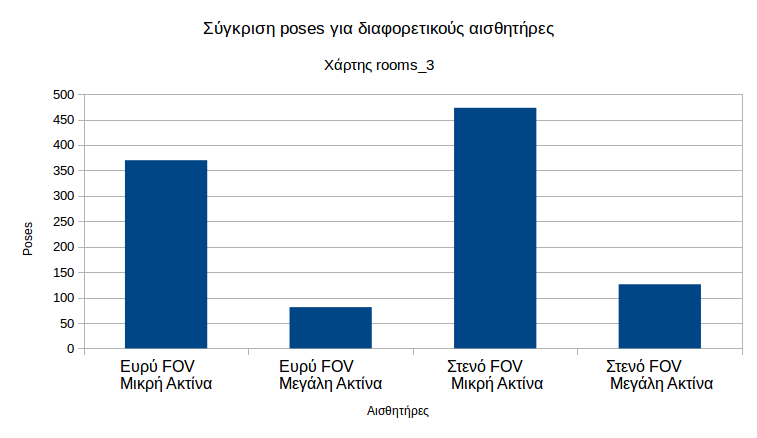
\includegraphics[width=\textwidth]{./images/chapter6/rooms_3_poses_compare.png}
         \label{fig:rooms_3_poses_compare}
         \caption{Σύγκριση αριθμών poses στον rooms\_3}
     \end{subfigure}
     \begin{subfigure}[b]{0.5\textwidth}
         \centering
         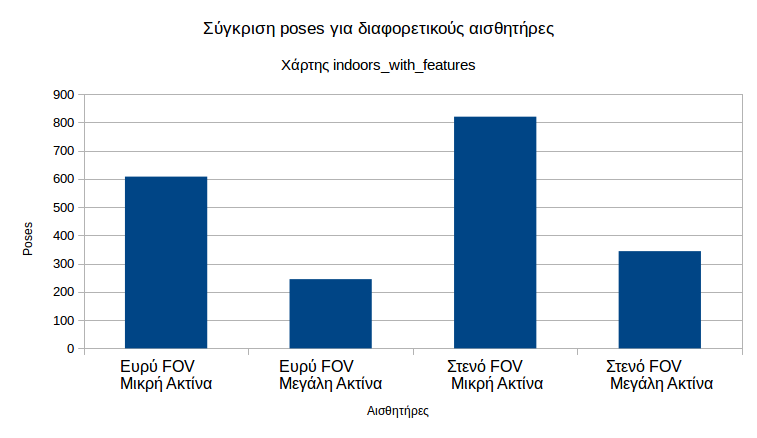
\includegraphics[width=\textwidth]{./images/chapter6/indoors_with_features_poses_compare.png}
         \label{fig:indoors_with_features_poses_compare}
         \caption{Σύγκριση αριθμών poses στον indoors\_with\_features}
     \end{subfigure}%
    %  -----------------------------------------
     \begin{subfigure}[b]{0.5\textwidth}
         \centering
         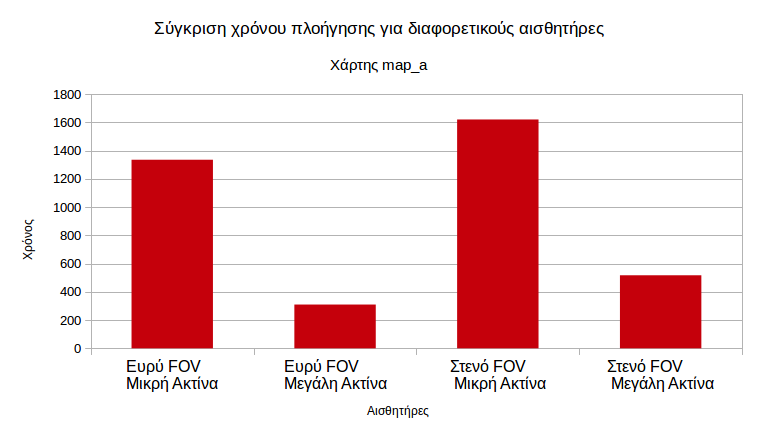
\includegraphics[width=\textwidth]{./images/chapter6/map_a_time_compare.png}
         \label{fig:map_a_time_compare}
         \caption{Σύγκριση χρόνου πλοήγησης στον map\_a}
     \end{subfigure}
     \begin{subfigure}[b]{0.5\textwidth}
         \centering
         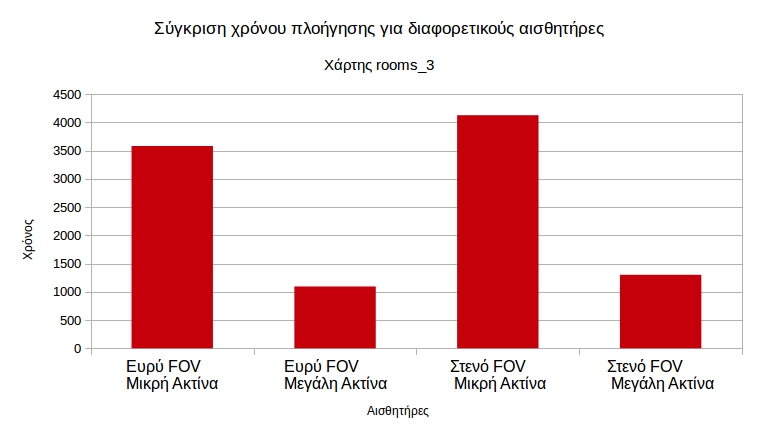
\includegraphics[width=\textwidth]{./images/chapter6/rooms_3_time_compare.png}
         \label{fig:rooms_3_time_compare}
         \caption{Σύγκριση χρόνου πλοήγησης στον rooms\_3}
     \end{subfigure}%
     \begin{subfigure}[b]{0.5\textwidth}
         \centering
         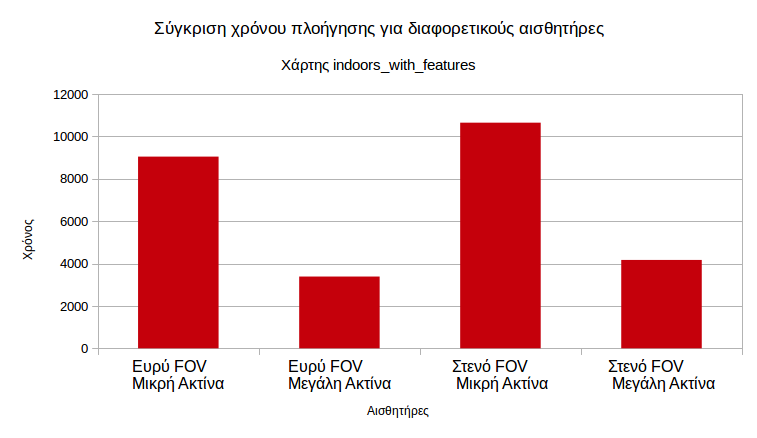
\includegraphics[width=\textwidth]{./images/chapter6/indoors_with_features_time_compare.png}
         \label{fig:indoors_with_features_time_compare}
         \caption{Σύγκριση χρόνου πλοήγησης στον indoors\_with\_features}
     \end{subfigure}
    %  ----------------------------------------------
\end{figure}
\begin{figure}[H]\ContinuedFloat
    \captionsetup{justification=centering}
    \begin{subfigure}[b]{0.5\textwidth}
         \centering
         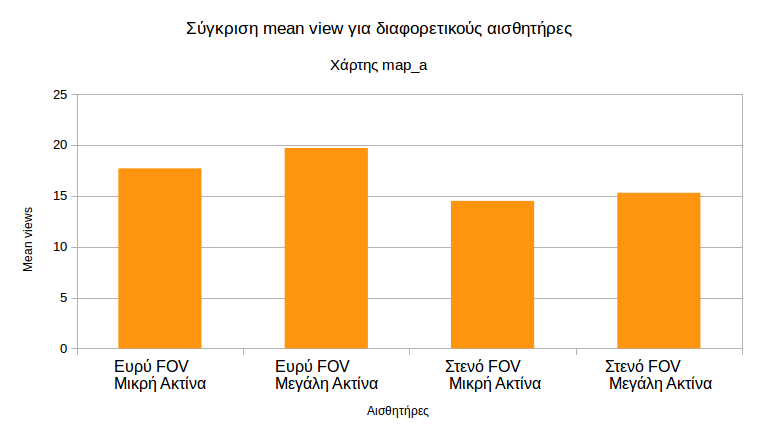
\includegraphics[width=\textwidth]{./images/chapter6/map_a_mean_views_compare.png}
         \label{fig:map_a_mean_views_compare}
         \caption{Σύγκριση mean views στον map\_a}
     \end{subfigure}%
     \begin{subfigure}[b]{0.5\textwidth}
         \centering
         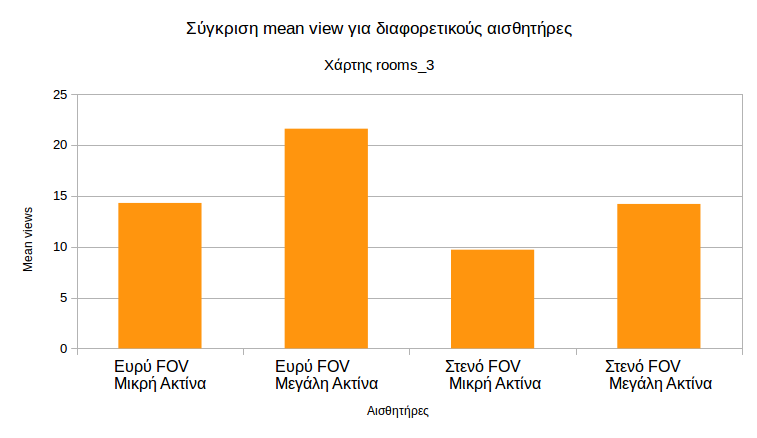
\includegraphics[width=\textwidth]{./images/chapter6/rooms_3_mean_views_compare.png}
         \label{fig:rooms_3_mean_views_compare}
         \caption{Σύγκριση mean views στον rooms\_3}
     \end{subfigure}
     \begin{subfigure}[b]{0.5\textwidth}
         \centering
         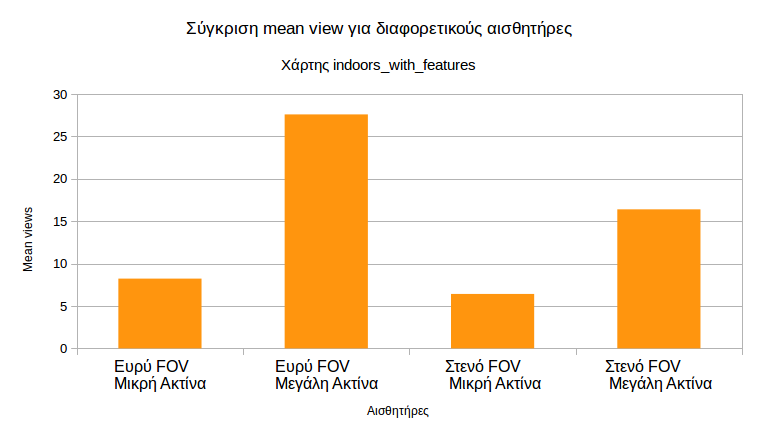
\includegraphics[width=\textwidth]{./images/chapter6/indoors_with_features_mean_views_compare.png}
         \label{fig:indoors_with_features_mean_views_compare}
         \caption{Σύγκριση mean views στον indoors\_with\_features}
     \end{subfigure}%
    \begin{subfigure}[b]{0.5\textwidth}
         \centering
         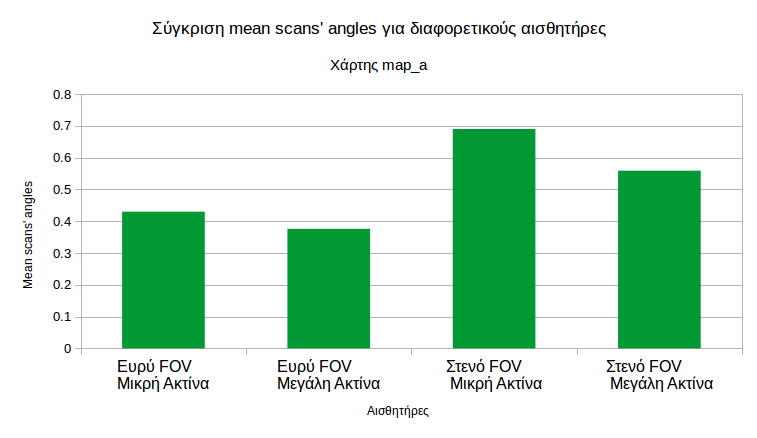
\includegraphics[width=\textwidth]{./images/chapter6/map_a_mean_angles_compare.png}
         \label{fig:map_a_mean_angles_compare}
         \caption{Σύγκριση mean scans' angles στον map\_a}
     \end{subfigure}
     \begin{subfigure}[b]{0.5\textwidth}
         \centering
         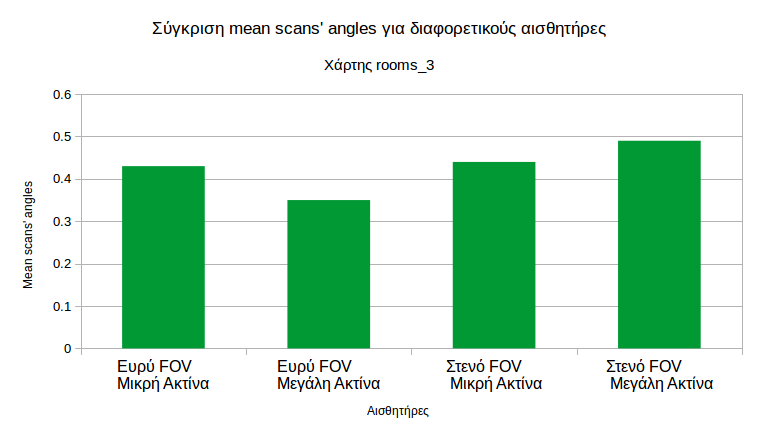
\includegraphics[width=\textwidth]{./images/chapter6/rooms_3_mean_angles_compare.png}
         \label{fig:rooms_3_mean_angles_compare}
         \caption{Σύγκριση mean scans' angles στον rooms\_3}
     \end{subfigure}%
     \begin{subfigure}[b]{0.5\textwidth}
         \centering
         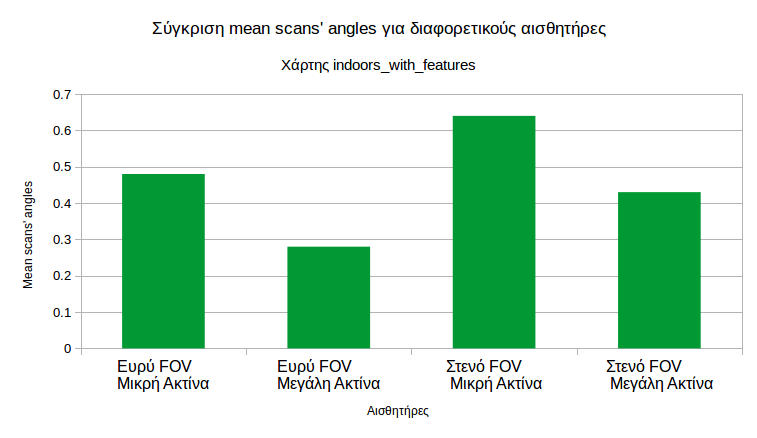
\includegraphics[width=\textwidth]{./images/chapter6/indoors_with_features_mean_angles_compare.png}
         \label{fig:indoors_with_features_mean_angles_compare}
         \caption{Σύγκριση mean scans' angles στον indoors\_with\_features}
     \end{subfigure}
     
     \caption{Σύγκριση αποτελεσμάτων για διαφορετικούς αισθητήρες με στρατηγική ακολουθίας τοίχων}
    \label{fig:sensors_compare}
\end{figure}

% \newpage

\begin{figure}[H]
     \centering
     \captionsetup{justification=centering}
     \begin{subfigure}[b]{\textwidth}
         \centering
         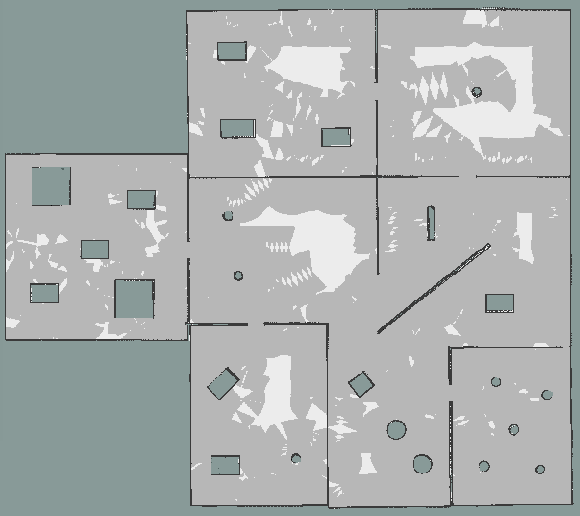
\includegraphics[width=0.6\textwidth]{./images/chapter6/indoors_with_features_wall_follow_coverage_narrow_short.png}
         \label{fig:indoors_with_features_wall_follow_coverage_narrow_short}
         \caption{Στενό FOV - Μικρή Ακτίνα}
     \end{subfigure}
     \begin{subfigure}[b]{\textwidth}
         \centering
         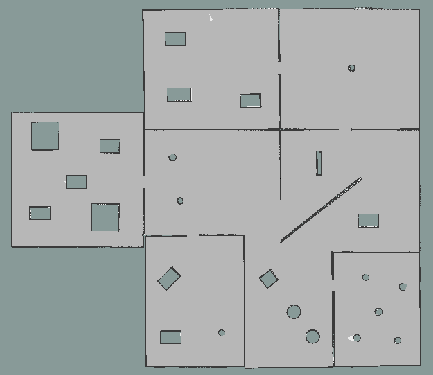
\includegraphics[width=0.6\textwidth]{./images/chapter6/indoors_with_features_wall_follow_coverage_wide_long.png}
         \label{fig:indoors_with_features_wall_follow_coverage_wide_long}
         \caption{Ευρύ FOV - Μεγάλη Ακτίνα}
     \end{subfigure}
     \caption{Πλήρης κάλυψη χάρτη indoors\_with\_features με στρατηγική ακολουθίας τοίχων για διαφορετικούς αισθητήρες}
    \label{fig:indoors_with_features_wall_follow_sensors_coverage_complare}
\end{figure}


Έπειτα, η χρήση σταθερού βήματος δειγματοληψίας, ανεξάρτητου από τα χαρακτηριστικά των αισθητήρων, έχει σημαντικές αρνητικές επιπτώσεις στη συνολική κάλυψη του χώρου. Στην περίπτωση που το βήμα είναι πολύ μεγαλύτερο από την ακτίνα των αισθητήρων η διαδικασία κάλυψης αποτυγχάνει πλήρως, όπως στο \autoref{fig:rooms_3_simple_large_coverage_wide_short}. Αντίθετα, στην περίπτωση που το βήμα δειγματοληψίας είναι πολύ μικρότερο από την ακτίνα των αισθητήρων ο συνολικός χρόνος κάλυψης αυξάνεται σημαντικά, φυσικά με εξαιρετικά αποτελέσματα κάλυψης, όπως φαίνονται και στο \autoref{fig:rooms_3_simple_small_coverage_narrow_long}. Συνεπώς, η αναπτυγμένη μέθοδος δειγματοληψίας με πολλαπλά βήματα με εξάρτηση από τα χαρακτηριστικά των αισθητήρων, οδηγεί σε μια συνολική βελτίωση της διαδικασίας ως προς την χρονική διάρκεια και την επιτυχία κάλυψης, όπως φαίνεται και στην πρόβλεψη κάλυψης \ref{fig:rooms_3_wall_follow_wide_long}, όπου και παρουσιάζονται τα σημεία - στόχοι, αλλά και στην τελική κάλυψη του χώρου \ref{fig:rooms_3_wall_follow_coverage_wide_long}. 



\begin{figure}[H]
     \centering
     \begin{subfigure}[b]{\textwidth}
         \centering
         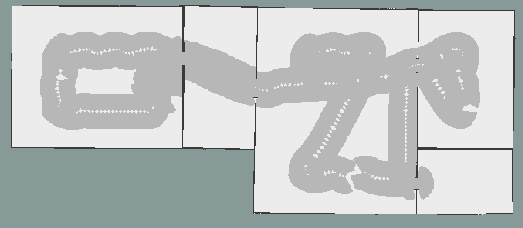
\includegraphics[width=0.6\textwidth]{./images/chapter6/rooms_3_simple_large_coverage_wide_short.png}
         \caption{Ευρύ FOV - Μικρή Ακτίνα με Απλή Στρατηγική μεγάλου βήματος δειγματοληψίας}
         \label{fig:rooms_3_simple_large_coverage_wide_short}
     \end{subfigure}
     \begin{subfigure}[b]{\textwidth}
         \centering
         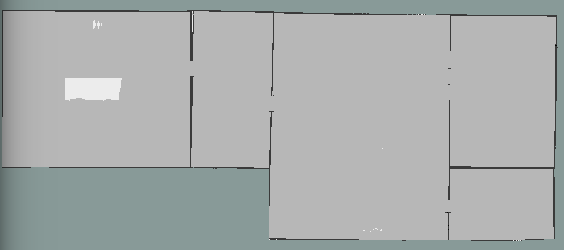
\includegraphics[width=0.6\textwidth]{./images/chapter6/rooms_3_simple_small_coverage_narrow_long.png}
         \caption{Στενό FOV - Μεγάλη Ακτίνα με Απλή Στρατηγική μικρού βήματος δειγματοληψίας}
         \label{fig:rooms_3_simple_small_coverage_narrow_long}
     \end{subfigure}
     \hfill
     \begin{subfigure}[b]{\textwidth}
         \centering
         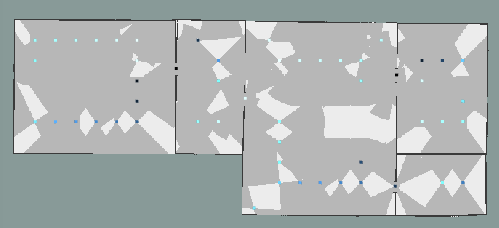
\includegraphics[width=0.6\textwidth]{./images/chapter6/rooms_3_wall_follow_wide_long.png}
         \caption{Ευρύ FOV - Μεγάλη Ακτίνα με στρατηγική ακολουθίας τοίχων, Πρόβλεψη Κάλυψης}
         \label{fig:rooms_3_wall_follow_wide_long}
     \end{subfigure}
\end{figure}
\begin{figure}[H]\ContinuedFloat
    \captionsetup{justification=centering}
     \begin{subfigure}[b]{\textwidth}
         \centering
         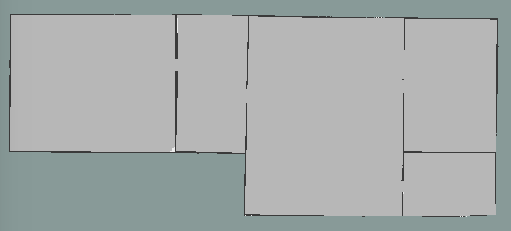
\includegraphics[width=0.6\textwidth]{./images/chapter6/rooms_3_wall_follow_coverage_wide_long.png}
         \caption{Ευρύ FOV - Μεγάλη Ακτίνα με στρατηγική ακολουθίας τοίχων}
         \label{fig:rooms_3_wall_follow_coverage_wide_long}
     \end{subfigure}
     \caption{Πλήρης κάλυψη χάρτη rooms\_3 με τις διάφορες στρατηγικές και διαφορετικούς αισθητήρες}
    \label{fig:rooms_3_sampling_coverage_results_compare}
\end{figure}

Τέλος, η στρατηγική zig zag συγκριτικά με τη wall follow αυξάνει μεν το πλήθος των σημείων και άρα τον συνολικό απαιτούμενο χρόνο, όμως αυξάνει κατά μέσο όρο και το πλήθος σαρώσεων των εμποδίων, ενώ στα περισσότερα πειράματα οι σαρώσεις είναι πιο ομοιόμορφες, ως αποτέλεσμα της μείωσης της μετρικής γωνίας σάρωσης. Συνεπώς, εαν η διαδικασία κάλυψης είναι ανάγκη να εκτελεστεί άμεσα και γρήγορα, μπορεί να επιλεγεί η στρατηγική ακολουθίας τοίχων, ενώ εαν είναι θεμιτό να καλυφθεί ο χώρος όσο το δυνατόν πιο αναλυτικά τότε μπορεί να επιλεγεί η στρατηγική ζιγκ ζαγκ.

Στο \autoref{fig:map_a_pattern_nodes_compare} παρουσιάζονται οι κόμβοι του χάρτη map\_a για τις δύο αυτές στρατηγικές. Σημειώνεται και η ακολουθία τους για κάθε δωμάτιο, η οποία εκκινεί από τα σκούρα σημεία και καταλήγει στα ανοικτόχρωμα, ενώ με μαύρο έχει τονιστεί η περιοχή που εκτιμάται ότι θα καλυφθεί από τα σημεία αυτά. 


\begin{figure}[H]
     \centering
     \captionsetup{justification=centering}
     \begin{subfigure}[b]{0.5\textwidth}
         \centering
         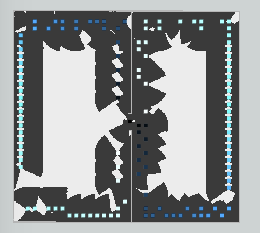
\includegraphics[width=0.8\textwidth]{./images/chapter6/map_a_wall_follow_wide_short.png}
         \label{fig:map_a_wall_follow_wide_short}
         \caption{Wall Follow Στρατηγική}
     \end{subfigure}%
     \begin{subfigure}[b]{0.5\textwidth}
         \centering
         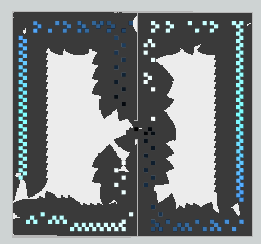
\includegraphics[width=0.8\textwidth]{./images/chapter6/map_a_zig_zag_wide_short.png}
         \label{fig:map_a_zig_zag_wide_short}
         \caption{Ζιγκ Ζαγκ Στρατηγική}
     \end{subfigure}
     \caption{Στόχοι και εκτίμηση κάλυψης του χάρτη map\_a για δύο στρατηγικές με Ευρύ FOV - Μικρή Ακτίνα}
    \label{fig:map_a_pattern_nodes_compare}
\end{figure}


